%%%%%%%%%%%%%%%%%%%%%%%%%%%%%%%%%%%%%%%%%%%%%%%%%%%%%%%%%%%%%%%%%%%%%%%%%%%%%%%%%%
\begin{frame}[fragile]\frametitle{}
\begin{center}
{\Large Let's not XAI}

\tiny{(Ref: Please Stop Doing ``Explainable'' ML - Cynthia Rudin  )}

\end{center}
\end{frame}

%%%%%%%%%%%%%%%%%%%%%%%%%%%%%%%%%%%%%%%%%%%%%%%%%%%%%%%%%%%
\begin{frame}[fragile]\frametitle{Distinction}

Although treated synonymously by many \ldots

\begin{itemize}
\item Explainable AI : model is a black-box and you explain it later (posthoc)
\item Interpretable AI: model itself is explanatory
\end{itemize}

\end{frame}

%%%%%%%%%%%%%%%%%%%%%%%%%%%%%%%%%%%%%%%%%%%%%%%%%%%%%%%%%%%
\begin{frame}[fragile]\frametitle{Accuracy vs Interpretability Plot}



\begin{columns}
    \begin{column}[T]{0.6\linewidth}
		
			\begin{itemize}
			\item Common myth peddled around
			\item More accurate the ML method is, lesser is its interpretability
			\item Argument: for any method, the whole attempt is to iteratively improve accuracy by understanding the data and the algorithm. Once settle many methods give similar accuracies.
			\item It may be possible to build interpretable ML model with accuracies similar to black box Deep Learning model (?)
			\end{itemize}
			
    \end{column}
    \begin{column}[T]{0.4\linewidth}

      \begin{center}
      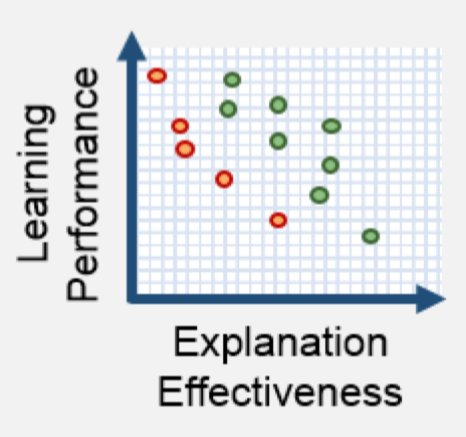
\includegraphics[width=\linewidth,keepaspectratio]{xai28}
	  	\end{center}
    \end{column}
  \end{columns}

\end{frame}

%%%%%%%%%%%%%%%%%%%%%%%%%%%%%%%%%%%%%%%%%%%%%%%%%%%%%%%%%%%
\begin{frame}[fragile]\frametitle{Flawed}

Why XAI is flawed?

\begin{columns}
    \begin{column}[T]{0.6\linewidth}
		
			\begin{itemize}
			\item You have your original model and the other surrogate explainable model.
			\item Both are different. They will disagree, even if thats 20\%, thats bad.
			\item Saliency Map in computer vision shows the area which helped the decision. But How helpful is that!! Still not sure what exactly made the decision, right?
			\end{itemize}
			
    \end{column}
    \begin{column}[T]{0.4\linewidth}

      \begin{center}
      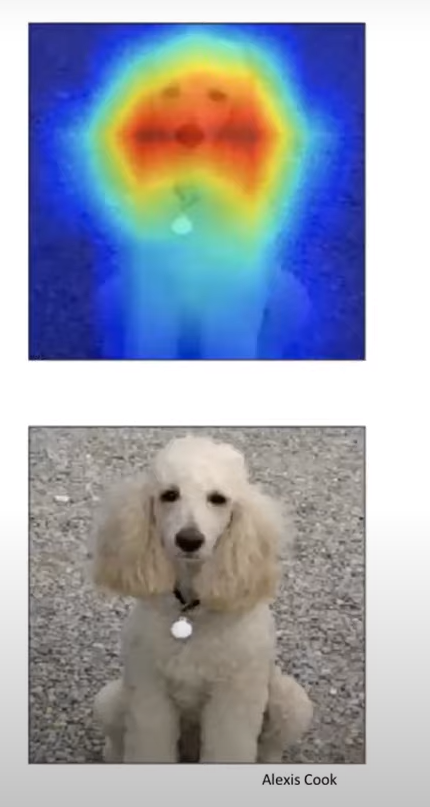
\includegraphics[width=0.8\linewidth,keepaspectratio]{xai29}
	  	\end{center}
    \end{column}
  \end{columns}

\end{frame}

%%%%%%%%%%%%%%%%%%%%%%%%%%%%%%%%%%%%%%%%%%%%%%%%%%%%%%%%%%%
\begin{frame}[fragile]\frametitle{Black boxes}

People love black boxes \ldots

\begin{itemize}
\item Companies can make money
\item Researchers do not have to put efforts in thoughtful and expensive feature engineering
\end{itemize}

Bottom-line: Teach, build and use interpretable ML models than black-box Deep Learning mdoels.

\end{frame}
